\section{Señales y procesamiento de señales}
	
	Una señal se define como cualquier cantidad física que varía con el tiempo, espacio o cualquier otra variable independiente. Un ejemplo de una señal es un electrocardiograma (ECG). Dicha señal le proporciona al médico información sobre el estado del corazón del paciente. De manera similar, una señal de electroencefalograma (EEG) proporciona información sobre la actividad del cerebro. \\
	
	Señales de audio, electrocardiograma y electroencefalograma son ejemplos de señales portadoras de información que evolucionan como funciones de una sola variable independiente, el tiempo. \\
	
	El procesamiento de la señal digital de la señal proporciona un método alternativo para procesar la señal analógica, para realizar el procesamiento digitalmente, se necesita una interfaz entre la señal analógica y el procesador digital. Esta interfaz se denomina convertidor analógico-digital(ADC). La salida del ADC es una señal digital apropiada como entrada del procesador digital. \\
	
	El procesador de señales digitales puede ser una gran computadora digital programable o un pequeño microprocesador programado para realizar las operaciones deseadas en la señal de entrada. \\
	
	Las señales digitales se almacenan fácilmente en medios magnéticos sin deterioro o pérdida de fidelidad de la señal más allá de la introducida en la conversión analógica-digital. \\
	
	Como consecuencia, las señales se vuelven transportables y pueden procesarse en cualquier lugar. El método de procesamiento de señales digitales también permite la implementación de algoritmos de procesamiento de señales más sofisticados. Por lo general, es muy difícil realizar operaciones matemáticas precisas en señales en forma analógica, pero estas mismas operaciones pueden implementarse fácilmente en software. \\
	
	En algunos casos, una implementación digital del sistema de procesamiento de señales es más barata que su contraparte analógica. El menor costo puede deberse al hecho de que el hardware digital es más barato o la flexibilidad para las modificaciones provistas por la implementación digital. \\
	
	Debido a estas ventajas, el procesamiento digital de señales se ha aplicado en sistemas prácticos que cubren una amplia gama de disciplinas. \cite{proakis} \\
	
	Dicho esto, se puede clasificar a las señales de dos maneras: analógica o digital. Una señal analógica es una forma de onda continua que cambia suavemente en el tiempo. A medida que las ondas se mueven desde el origen hasta el destino, la onda va a adquiriendo un número infinito de valores en su camino. Por el contrario, una señal digital es discreta. Solamente puede tener un número de valores definidos, a menudo tan simples como son los estados binarios cero y uno. \cite{signal} \\
			
	Un ejemplo de estas señales se muestra en la figura \ref{fig:analog-digital}. La señal con fondo negro es una señal analógica, por lo que presenta valores continuos. La señal de fondo blanco es la representación digital de la anterior. \\
	
	\begin{figure}[htbp!]
		\centering
		\fbox{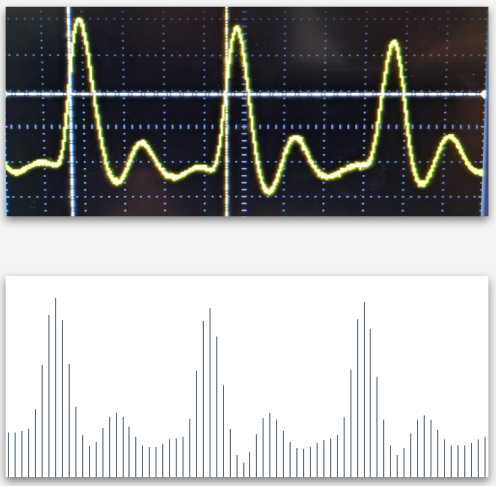
\includegraphics[width=0.7\textwidth]{MarcoTeorico/imagenes/analog-digital.png}}
		\caption{Señal analógica y señal digital.}
		\label{fig:analog-digital}
	\end{figure}
	
	\subsection{Teorema de muestreo}
	El teorema de muestreo especifica la frecuencia mínima a la que se debe muestrear uniformemente una señal de tiempo continuo para que la señal original pueda ser recuperada o reconstruida por completo solo con estas muestras. El muestreo es el número de lecturas completadas cada segundo. \\
	
	Si una señal de tiempo continuo no contiene componentes de frecuencia superiores a $w$ Hz, entonces puede determinarse completamente mediante muestras uniformes tomadas a una frecuencia de $fs$ muestras por segundo donde:
	$$fs \geq 2w$$
	
	La frecuencia de muestreo mínima permitida por el teorema de muestreo ($fs = 2w$) se denomina tasa de Nyquist. \cite{sampling}
	
	\subsection{Análisis de señales}
	
	\subsubsection{Autocorrelación}
	La autocorrelación se aplica sobre la misma señal y es muy útil para conocer propiedades de la señal
	como por ejemplo si posee una frecuencia básica fundamental que es la responsable de las restantes. \\
	
	Existen dos estimaciones básicas de la autocorrelación:
	\begin{itemize}
		\item Estimación de la autocorrelación no parcial (Unbiased autocorrelation estimate).
		\item Estimación de la autocorrelación parcial (Biased autocorrelation estimate). \\
		Se expresa como:
		
		$$Cxx[n] = \frac{1}{N} \sum_{m=0}^{N-1-n}x[m]x[m+n]$$
		
		La respuesta de la función de autocorrelación estimada es positiva definida y el mayor
		valor se corresponde siempre con el origen. El máximo está en el origen y se corresponde con la
		energía de la señal, la diferencia del máximo inicial al segundo máximo representa la frecuencia fundamental de la señal, si éste está presente y existe.
	\end{itemize}

